%%%%%%%%%%%%%%%%%%%%%%%%%%%%%%%%%%%%%%%%%%%%%%%%%%%%%%%%%%%%%%%%%%%%%%%%%%%
%% This file is part of the book
%%
%% Algorithmic Graph Theory
%% http://code.google.com/p/graph-theory-algorithms-book/
%%
%% Copyright (C) 2009, 2010, 2011 Minh Van Nguyen <nguyenminh2@gmail.com>
%%
%% See the file COPYING for copying conditions.
%%%%%%%%%%%%%%%%%%%%%%%%%%%%%%%%%%%%%%%%%%%%%%%%%%%%%%%%%%%%%%%%%%%%%%%%%%%

%% hypercube graph Q_1
\subfigure[$Q_1$]{
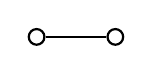
\begin{tikzpicture}
[nodedecorate/.style={shape=circle,inner sep=2pt,draw,thick},%
  linedecorate/.style={-,thick}]
%% nodes or vertices
\node (1) at (0,0) [nodedecorate] {};
\node (2) at (1,0) [nodedecorate] {};
%% edges or lines
\path
(1) edge[linedecorate] node {} (2);
\end{tikzpicture}
}
%%
%% hypercube graph Q_2
\subfigure[$Q_2$]{
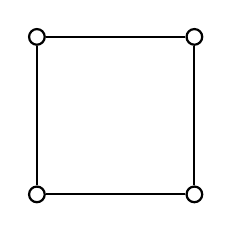
\begin{tikzpicture}
[nodedecorate/.style={shape=circle,inner sep=2pt,draw,thick},%
  linedecorate/.style={-,thick}]
%% nodes or vertices
\foreach \nodename/\x/\y in {1/0/0, 2/2/0, 3/2/2, 4/0/2} {
  \node (\nodename) at (\x,\y) [nodedecorate] {};
}
%% edges or lines
\path
\foreach \startnode/\endnode in {1/2, 2/3, 3/4, 4/1} {
  (\startnode) edge[linedecorate] node {} (\endnode)
};
\end{tikzpicture}
}
%%
%% hypercube graph Q_3
\subfigure[$Q_3$]{
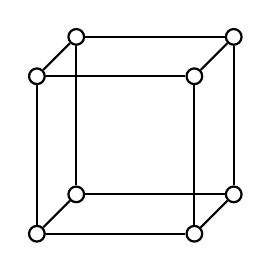
\begin{tikzpicture}
[nodedecorate/.style={shape=circle,inner sep=2pt,draw,thick},%
  linedecorate/.style={-,thick}]
%% nodes or vertices
\foreach \nodename/\x/\y in {1/0/0, 2/2/0, 3/2/2, 4/0/2, 5/0.5/0.5,
  6/2.5/0.5, 7/2.5/2.5, 8/0.5/2.5}
{
  \node (\nodename) at (\x,\y) [nodedecorate] {};
}
%% edges or lines
\path
\foreach \startnode/\endnode in {1/2, 2/3, 3/4, 4/1, 5/6, 6/7, 7/8,
  8/5, 1/5, 2/6, 3/7, 4/8}
{
  (\startnode) edge[linedecorate] node {} (\endnode)
};
\end{tikzpicture}
}
%%
%% hypercube graph Q_4
\subfigure[$Q_4$]{
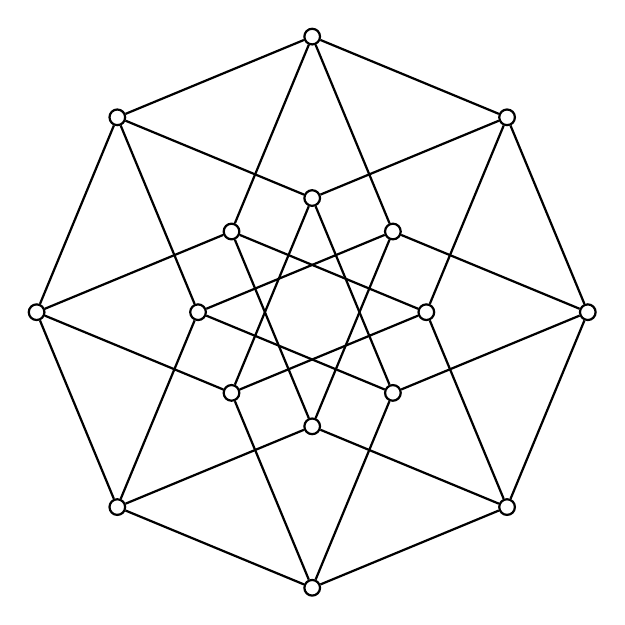
\begin{tikzpicture}
[nodedecorate/.style={shape=circle,inner sep=2pt,draw,thick},%
  linedecorate/.style={-,thick},%
  scale=3.5]
%% nodes or vertices
\foreach \nodename/\x/\y in {1/1/0, 2/0.7071/0.7071, 3/0/1,
  4/-0.7071/0.7071, 5/-1/0, 6/-0.7071/-0.7071, 7/0/-1,
  8/0.7071/-0.7071, 9/0.4142/0, 10/0.2928/0.2928, 11/0/0.4142,
  12/-0.2928/0.2928, 13/-0.4142/0, 14/-0.2928/-0.2928, 15/0/-0.4142,
  16/0.2928/-0.2928}
{
  \node (\nodename) at (\x,\y) [nodedecorate] {};
}
%% edges or lines
\path
\foreach \startnode/\endnode in {1/2, 1/8, 1/10, 1/16, 2/3, 2/9, 2/11,
  3/4, 3/10, 3/12, 4/5, 4/11, 4/13, 5/6, 5/12, 5/14, 6/7, 6/13, 6/15,
  7/8, 7/14, 7/16, 8/9, 8/15, 9/12, 9/14, 10/13, 10/15, 11/14, 11/16,
  12/15, 13/16}
{
  (\startnode) edge[linedecorate] node {} (\endnode)
};
\end{tikzpicture}
}
